\documentclass[12pt,twoside]{article}
\usepackage{light}
%\usepackage{tikz}
%\usepackage{bbding, manfnt, gensymb}
%\usepackage{pstricks}
\usepackage{verbatim}

\hidesolutions
\showsolutions

\newcommand{\hint}[1]{({\it Hint: #1})}
\newcommand{\card}[1]{\left|#1\right|}

\begin{document}
\problemset{7}{October 27, 2016}{Tuesday, November 1}
\newcommand{\proofrubric}[3][Any correct proof.]
  {
  	\begin{center}
	\fbox{\begin{minipage}{35em}
	\textbf{Rubric}
	\par
	[#3pts] #1
		\begin{center}
		\textbf{or}
		\end{center}
	#2
	\end{minipage}}
	\end{center}
  }
  
  \newcommand{\proofrubriceach}[3][Any correct proof.]
  {
  	\begin{center}
	\fbox{\begin{minipage}{35em}
	\textbf{Rubric For Each}
	\par
	[#3pts] #1
		\begin{center}
		\textbf{or}
		\end{center}
	#2
	\end{minipage}}
	\end{center}
  }
  
  \newcommand{\rubric}[1]
  {
  	\begin{center}
	\fbox{\begin{minipage}{35em}
	\textbf{Rubric}
	\par
	#1
	\end{minipage}}
	\end{center}
  }


\begin{problem}{15}
 Express
\[
 \sum_{i=0}^n i^2x^i
\]
as a closed-form function of $n$.
\proofrubric[Any correct result with some work shown.]{
[5pts] Start out with formula from lecture. \par
[5pts] Differentiating both sides. \par
[5pts] Multiplying both sides by $x$. \par
[-1pt] Math errors.
}{15}

\solution{
We use the derivative method. Let us start with the following formula, derived in lecture (for $x \not= 1$):

\[
 \sum_{i=0}^n ix^i = \frac{x-(n+1)x^{n+1} + nx^{n+2}}{(1-x)^2}
\]

Differentiating both sides:

\begin{align*}
 x^{-1}\sum_{i=0}^n i^2x^i =& \frac{(1-(n+1)^2x^n + n(n+2)x^{n+1})(1-x)^2 - (x-(n+1)x^{n+1}+nx^{n+2})(2(1-x)(-1))}{(1-x)^4} \\
 =&  \frac{(1-(n+1)^2x^n + n(n+2)x^{n+1})(1-x) +2 (x-(n+1)x^{n+1}+nx^{n+2})}{(1-x)^3} \\
 =&  \frac{1-(n+1)^2x^n + n(n+2)x^{n+1} - x + (n+1)^2x^{n+1} - n(n+2)x^{n+2}}{(1-x)^3} \\
 &+ \frac{2x - 2(n+1)x^{n+1} + 2nx^{n+2}}{(1-x)^3} \\
 =& \frac{1 + x - (n+1)^2x^n + (n(n+2) + (n+1)^2 - 2(n+1))x^{n+1}   + (2n - n(n+2))x^{n+2}}{(1-x)^3} \\
 =& \frac{1 + x - (n+1)^2x^n + (2n^2+2n-1)x^{n+1} - n^2x^{n+2}}{(1-x)^3}.
\end{align*}

Multiplying both sides by $x$, we get
\[
 \sum_{i=0}^n i^2x^i = \frac{x(1 + x - (n+1)^2x^n + (2n^2+2n-1)x^{n+1} - n^2x^{n+2})}{(1-x)^3}.
\]
}


\end{problem}


\begin{problem}{20}
\proofrubriceach[Any correct result with some work shown.]{
[3pts] Simplify expression into manageable summations. \par
[2pts] Simplifying summations.\par
[-1pt] Math errors.
}{5}
\bparts
\ppart{5}
What is the product of the first $n$ odd powers of two: $\prod\limits_{k=1}^n2^{2k-1}$?   
\
\medskip
\solution{ 
\[
\Pi_{k=1}^n2^{2k-1} = 2^{\sum_{k=1}^n{2k-1}}
= 2^{2\sum_{k=1}^n k-\sum_{k=1}^n 1}
= 2^{n(n+1) - n}
= 2^{n^2}
\]
}
%\vspace*{2in}

\ppart{5}
Find a closed expression for 
\[
\sum_{i=0}^n \sum_{j=0}^m 3^{i+j}
\]

\solution{
\begin{align*}
\sum_{i=0}^n \sum_{j=0}^m 3^{i+j}
    & = \sum_{i=0}^n \left(3^i \cdot \sum_{j=0}^m 3^j\right) \\
    & = \left(\sum_{j=0}^m 3^j\right) \cdot \left(\sum_{i=0}^n 3^i\right)\\
    & = \left(\frac{3^{m+1} - 1}{2}\right) \cdot \left(\frac{3^{n+1} - 1}{2}\right)
\end{align*}
}

\ppart{5}
Find a closed expression for
\[
\sum_{i=1}^n \sum_{j=1}^n (i + j)
\]

\solution{
\begin{align*}
\sum_{i=1}^n \sum_{j=1}^n (i + j)
    & = \left (\sum_{i=1}^n \sum_{j=1}^n i \right ) + \left (\sum_{i=1}^n \sum_{j=1}^n j \right )\\
    & = \left (\sum_{i=1}^n ni \right ) + \left (\sum_{i=1}^n  \frac{n(n+1)}{2} \right )\\
    & = \frac{2n^2(n+1)}{2}\\
    & = n^2(n+1)
\end{align*}
}

\ppart{5}
Find a closed expression for
\[
 \prod_{i=1}^n \prod_{j=1}^n 2^i \cdot 3^j
\]

\solution{
\begin{align*}
\prod_{i=1}^n \prod_{j=1}^n 2^i \cdot 3^j
    & = \left (\prod_{i=1}^n 2^{ni} \right ) \left (\prod_{j=1}^n 3^{nj} \right )\\
    & = 2^{n\sum_{i=1}^n i}3^{n\sum_{j=1}^n j}\\
    & = 2^{n^2(n+1)/2}3^{n^2(n+1)/2}
\end{align*}
}

\eparts

\end{problem}

\begin{problem}{10}
\bparts
\ppart{6}
Use integration to find upper and lower bounds that differ by at most
0.1 for the following sum.  (You may need to add the first few terms
explicitly and then use integrals to bound the sum of the remaining
terms.)
\rubric{
[2pts] Use integrals to estimate. \par
[2pts] Realize the need to sum the first few terms explicitly and bound the rest with integrals. \par
[2pts] Bounds differ by at most 0.1.
}
%
\[
\sum_{i=1}^{\infty} \frac{1}{(2i+1)^2}
\]

\solution{
Let's first try standard bounds:
%
\[
\int_1^{\infty} \frac{1}{(2x+1)^2}\ dx
\quad \leq \quad
\sum_{i=1}^{\infty} \frac{1}{(2i+1)^2}
\quad \leq \quad
f(1) + \int_1^{\infty} \frac{1}{(2x+1)^2}\ dx
\]
%
Evaluating the integrals gives:
%
\[
\left. -\frac{1}{2(2x+1)}\ \right|_1^{\infty}
\quad \leq \quad
\sum_{i=1}^{\infty} \frac{1}{(2i+1)^2}
\quad \leq \quad
\left. \frac{1}{3^2}+ -\frac{1}{2 (2x+1)}\ \right|_1^{\infty}
\]
%
\[
\frac{1}{6}
\quad \leq \quad
\sum_{i=1}^{\infty} \frac{1}{(2i+1)^2}
\quad \leq \quad
\frac{1}{9}+\frac{1}{6}
\]
%
These bounds are too far apart, so let's sum the first couple terms
explicitly and bound the rest with integrals.
%
\[
\frac{1}{3^2} + \int_2^{\infty} \frac{1}{(2x+1)^2}\ dx
\quad \leq \quad
\sum_{i=1}^{\infty} \frac{1}{(2i+1)^2}
\quad \leq \quad
\frac{1}{3^2} + f(2) + \int_2^{\infty} \frac{1}{(2x+1)^2}\ dx
\]
%
Integration now gives:
%
\[
\frac{1}{3^2} +  \left(\left. - \frac{1}{2 (2x+1)}\ \right|_2^{\infty}\right)
\quad \leq \quad
\sum_{i=1}^{\infty} \frac{1}{(2i+1)^2}
\quad \leq \quad
\frac{1}{3^2} + \frac{1}{5^2} + 
    \left(\left. - \frac{1}{2 (2x+1)}\ \right|_2^{\infty}\right)
\]
\[
\frac{1}{3^2} + \frac{1}{10}
\quad \leq \quad
\sum_{i=1}^{\infty} \frac{1}{(2i+1)^2}
\quad \leq \quad
\frac{1}{3^2} + \frac{1}{5^2} + \frac{1}{10}
\]
%
Now we have bounds that differ by $1/5^2 = 0.04$.
}

\ppart{4}
Assume $n$ is an integer larger than 1. Which of the following inequalities, if any, hold.  You may find the graph helpful. 

\begin{figure}[h]
\begin{center}
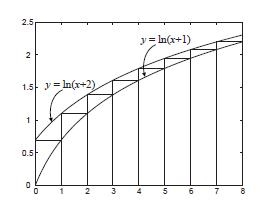
\includegraphics[width=3in,clip]{integral}
\end{center}
\end{figure}
\rubric{
[2pts] 1st inequality holds. \par
[2pts] 2nd inequality does not hold.
}
\begin{enumerate}

\item $\displaystyle \sum_{i=1}^n \ln (i+1) \le \int_0^n \ln(x+2)
dx $

\item $\displaystyle \sum_{i=1}^n \ln (i+1) \le \ln 2 + \int_1^n
\ln(x+1) dx $

\end{enumerate}

\solution{The 1st inequality holds.}
\eparts

\end{problem}



%\begin{problem}{15}
%There is a bug on the edge of a 1-meter rug.  The bug wants to cross
%to the other side of the rug.  It crawls at 1 cm per second.  However,
%at the end of each second, a malicious first-grader named Mildred
%Anderson \textit{stretches} the rug by 1 meter.  Assume that her
%action is instantaneous and the rug stretches uniformly.  Thus, here's
%what happens in the first few seconds:
%
%\begin{itemize}
%
%\item The bug walks 1 cm in the first second, so 99 cm remain ahead.
%
%\item Mildred stretches the rug by 1 meter, which doubles its length.
%So now there are 2 cm behind the bug and 198 cm ahead.
%
%\item The bug walks another 1 cm in the next second, leaving 3 cm
%behind and 197 cm ahead.
%
%\item Then Mildred strikes, stretching the rug from 2 meters to 3
%meters.  So there are now $3 \cdot (3 / 2) = 4.5$ cm behind the bug
%and $197 \cdot (3/2) = 295.5$ cm ahead.
%
%\item The bug walks another 1 cm in the third second, and so on.
%
%\end{itemize}
%
%Your job is to determine this poor bug's fate.
%
%\bparts
%
%\ppart{5}
%During second $i$, what \textit{fraction} of the rug does the
%bug cross?
%
%\solution{During second $i$, the length of the rug is $100i$ cm and
%the bug crosses 1 cm.  Therefore, the fraction that the bug crosses is
%$1 / 100i$.}
%
%\ppart{5}
%Over the first $n$ seconds, what fraction of the rug does the bug cross altogether?  Express your answer in terms of the Harmonic number $H_n$.
%
%\solution{The bug crosses $1/100$ of the rug in the first second,
%$1/200$ in the second, $1/300$ in the third, and so forth.  Thus, over
%the first $n$ seconds, the fraction crossed by the bug is:
%%
%\[
%\sum_{k=1}^{n} \frac{1}{100k} = H_n / 100
%\]
%%
%(This formula is valid only until the bug reaches the far side of the
%rug.)}
%
%\ppart{5}
%Approximately how many seconds does the bug need to cross the
%entire rug?
%
%\solution{The bug arrives at the far side when the fraction it has
%crossed reaches 1.  This occurs when $n$, the number of seconds
%elapsed, is sufficiently large that $H_n / 100 \geq 1$.  Now $H_n$ is
%approximately $\ln n$, so the bug arrives about when:
%%
%\begin{align*}
%\frac{\ln n}{100} & \geq 1 \\
%\ln n & \geq 100 \\
%n & \geq e^{100} \approx 10^{43} \text{ seconds}
%\end{align*}
%}
%
%\eparts
%
%\end{problem}

\begin{problem}{20}
For each of the following six pairs of functions $f$ and $g$ (parts (a) through (f)), state which of these order-of-growth relations hold (more than one may hold, or none may hold):
\proofrubriceach[Correct list of relations]{
[0pts] No relation correct. \par
[-2pts] Each missed relation (caps at -5pts). \par
[-2pts] Each extra relation (caps at -5pts).
}{5}
\begin{align*}
 f = o(g) && f=O(g) && f=\omega(g) && f=\Omega(g) && f=\Theta(g) && f \sim g
\end{align*}

\begin{align*}
\textbf{(a)}&& f(n) &= \log_2 n &  g(n) &= \log_{10} n \\
\textbf{(b)}&& f(n) &= 2^n & g(n) &= 10^n\\
\textbf{(c)}&& f(n) &= 0 & g(n) &= 17\\
\textbf{(d)}&& f(n) &= 1+\cos\left(\frac{\pi n}{2}\right) & g(n) &= 1+\sin\left(\frac{\pi n}{2}\right)\\
\textbf{(e)}&& f(n) &= {1.0000000001}^n & g(n) &= n^{10000000000}\\
\end{align*}

\solution{
 \begin{itemize}
  \item $f(n) = \log_2 n$ and $g(n) = \log_{10} n$:
\begin{align*}
   	\lim_{n\to\infty} \left|\frac{f(n)}{g(n)}\right|
	&= \lim_{n\to\infty}\frac{\ln n / \ln 2}{\ln n / \ln 10} \\
	&= \frac{\ln 10}{\ln 2}
  \end{align*}
	 So $f(n) = \Omega(g(n))$ and $f(n) = O(g(n))$ and $f(n) = \Theta(g(n))$.

  \item $f(n) = 2^n$ and $g(n) = 10^n$:
\begin{align*}
   	\lim_{n\to\infty} \left|\frac{f(n)}{g(n)}\right|
	&= \lim_{n\to\infty} \frac{2^n}{10^n} \\
	&= \lim_{n\to\infty} (1/5)^n \\
	&= 0
  \end{align*}
	 So $f(n) = o(g(n))$ and $f(n) = O(g(n))$.

\item $f(n) = 0$ and $g(n) = 17$:
\begin{align*}
   	\lim_{n\to\infty} \left|\frac{f(n)}{g(n)}\right|
	&= \frac{0}{17} \\
	&= 0
  \end{align*}
	 So $f(n) = o(g(n))$ and $f(n) = O(g(n))$.

\item $f(n) = 1+\cos\left(\frac{\pi n}{2}\right)$ and $g(n) = 1+\sin\left(\frac{\pi n}{2}\right)$:

	For all $n \equiv 1$ (mod 4), $f(n)/g(n) = 0$, so $f(n) \not= \Omega(g(n))$. Likewise, for all $n \equiv 0$ (mod 4), 
$g(n)/f(n) = 0$, so $f(n) \not= O(g(n))$.  The quotient never converges to some particular limit, so no relation holds.

\item $f(n) = {1.0000000001}^n$ and $g(n) = n^{10000000000}$:
\begin{align*}
   	\lim_{n\to\infty} \left|\frac{f(n)}{g(n)}\right|
	&= \lim_{n\to\infty} \frac{1.0000000001^n}{n^{10000000000}} \\
	&= \lim_{n\to\infty} \frac{1.0000000001^n \ln 1.0000000001}{10000000000n^{9999999999}} \\
	&= \lim_{n\to\infty} \frac{1.0000000001^n (\ln 1.0000000001)^{10000000000}}{10000000000!} \\
	&= \infty
  \end{align*}
	 So $f(n) = \omega(g(n))$ and $f(n) = \Omega(g(n))$.

	
 \end{itemize}

}
\end{problem}

%\begin{problem}{15}
%This problem continues the study of the asymptotics of factorials.
%\bparts
%\ppart{5}
%
%Either prove or disprove each of the following statements.
%\begin{itemize}
%\item $n! = O((n+1)!)$
%\item $n! = \Omega((n+1)!)$
%\item $n! = \Theta((n+1)!)$
%\item $n! = \omega((n+1)!)$
%\item $n! = o((n+1)!)$
%\end{itemize}
%
%\solution{Observe that $n! = (n+1)!/(n+1)$, and thus $n! = o((n+1)!)$. Thus, $n! = O((n+1)!)$ as well, but the remaining statements are false.}
%
%\ppart{5}
%Show that $n! = \omega \left( \left (\frac{n}{3} \right )^{n+e} \right)$.
%
%\solution{By Stirling's formula:
%\[
%n! \sim \sqrt{2 \pi n} \left(\frac{n}{e}\right)^{n}
%\]
%
%On the other hand, note that $\left (\frac{n}{3} \right )^{n+e} = \left (\frac{n}{3} \right )^e \left (\frac{n}{3} \right )^n$. Dividing $n!$ by this quantity,
%$$\frac{3^e\sqrt{2\pi}}{n^{e-1/2}} \cdot \left (\frac{3}{e} \right )^n,$$
%we see that since $3 > e$, this expression goes to $\infty$. Thus, $n! = \omega \left (\frac{n}{3} \right )^{n+e}$.
%}
%
%\ppart {5}
%Show that $n! = \Omega(2^n)$
%\solution{
%We can proceed straight from the definition. Recall $n!$  is $\Omega\left(2^n\right)$ if and only if 
%
%$$\lim_{n \to \infty} \dfrac{n!}{2^n} > 0$$
%
% 
%By multiplying and dividing by the same factor, we get
%
%$$\lim_{n \to \infty} \dfrac{n!}{2^n} = \lim_{n \to \infty} \dfrac{n!}{\left( \dfrac{n}{e}\right)^n \sqrt{2\pi n}} \dfrac{\left( \dfrac{n}{e}\right)^n \sqrt{2\pi n}}{2^n}$$
%
%And using Stirling's approximation, we know the left part tends to 1. So we only need to worry about 
%
%$$\lim_{n \to \infty} \dfrac{\left( \dfrac{n}{e}\right)^n \sqrt{2\pi n}}{2^n}$$
%
%The expression in the limit can be manipulated to be 
%
%$$\left( \dfrac{n}{2e}\right)^n \sqrt{2\pi n}$$
%
%Since $n^n$ is strictly larger than $10^n$ for $n > 10$, then 
%
%$$\lim_{n \to \infty} \left( \dfrac{n}{2e}\right)^n \sqrt{2\pi n} >  \lim_{n \to \infty} \left( \dfrac{10}{2e} \right)^n \sqrt{2\pi n} = \infty$$
%
%So the original limit must also be $\infty$. This also shows that in fact $n! = \omega \left(2^n \right)$ And the same argument can be used to show that $n! = \omega \left(10^n\right)$ or any other constant base.
%
%}
%\eparts
%\end{problem}

\end{document}
